\let\negmedspace\undefined
\let\negthickspace\undefined
\documentclass[journal]{IEEEtran}
\usepackage[a5paper, margin=10mm, onecolumn]{geometry}
%\usepackage{lmodern} % Ensure lmodern is loaded for pdflatex
\usepackage{tfrupee} % Include tfrupee package

\setlength{\headheight}{1cm} % Set the height of the header box
\setlength{\headsep}{0mm}     % Set the distance between the header box and the top of the text

\usepackage{gvv-book}
\usepackage{gvv}
\usepackage{cite}
\usepackage{amsmath,amssymb,amsfonts,amsthm}
\usepackage{algorithmic}
\usepackage{graphicx}
\usepackage{textcomp}
\usepackage{xcolor}
\usepackage{txfonts}
\usepackage{listings}
\usepackage{enumitem}
\usepackage{mathtools}
\usepackage{gensymb}
\usepackage{comment}
\usepackage[breaklinks=true]{hyperref}
\usepackage{tkz-euclide} 
\usepackage{listings}
% \usepackage{gvv}                                        
\def\inputGnumericTable{}                                 
\usepackage[latin1]{inputenc}                                
\usepackage{color}                                            
\usepackage{array}                                            
\usepackage{longtable}                                       
\usepackage{calc}                                             
\usepackage{multirow}                                         
\usepackage{hhline}                                           
\usepackage{ifthen}                                           
\usepackage{lscape}
\usepackage{circuitikz}
\tikzstyle{block} = [rectangle, draw, fill=blue!20, 
    text width=4em, text centered, rounded corners, minimum height=3em]
\tikzstyle{sum} = [draw, fill=blue!10, circle, minimum size=1cm, node distance=1.5cm]
\tikzstyle{input} = [coordinate]
\tikzstyle{output} = [coordinate]


\begin{document}

\bibliographystyle{IEEEtran}
\vspace{3cm}

\title{2.7.25}
\author{EE25BTECH11013 - Bhargav}
\maketitle
% \newpage
% \bigskip
{\let\newpage\relax\maketitle}

\renewcommand{\thefigure}{\theenumi}
\renewcommand{\thetable}{\theenumi}
\setlength{\intextsep}{10pt} % Space between text and floats


\numberwithin{equation}{enumi}
\numberwithin{figure}{enumi}
\renewcommand{\thetable}{\theenumi}

\textbf{Question}:\\
Find the area of quadrilateral $ABCD$ whose vertices are  $A(-3,-1)$, $B(-2,-4)$, $C(4,-1)$ and $D(3,4)$. \\
\solution\\
The area of the quadrilateral can be found by dividing it into 2 triangles and adding them to find the area of the quadrilateral.
The area of triangle $ABC$ and $ACD$ can be computed separately. \\ \\

\begin{align}
\vec{A} = \myvec{-3 \\ -1}
\end{align}
\begin{align}
\vec{B} = \myvec{-2 \\ -4}
\end{align}
\begin{align}
\vec{C} = \myvec{4 \\ -1}
\end{align}
\begin{align}
\vec{D} = \myvec{3 \\ 4}
\end{align}



Choose \(\vec{A}\) as a common vertex and form vectors for triangles ABC and ACD.


\begin{align}
\vec{A}-\vec{B} 
= \myvec{-3+2 \\ -1+4} = \myvec{-1 \\ 3}
\end{align}


\begin{align}
\vec{A} - \vec{C} = \myvec{-3-4 \\ -1+1} = \myvec{-7 \\ 0}
\end{align}



\begin{align}
(\triangle ABC)=\frac{1}{2}\norm{(\vec{A}-\vec{B}) \times (\vec{A}-\vec{C})}
\end{align}

\begin{align}
(\triangle ABC)=\frac{1}{2}\norm{\myvec{-1 \\ 3} \times \myvec{-7 \\ 0}}=\frac{1}{2}\cdot 21=\frac{21}{2}.
\end{align}


\begin{align}
\vec{A}-\vec{D}
=\myvec{-3-3 \\ -1-4} = \myvec{-6 \\ -5}  
\end{align}





\begin{align}
(\triangle ACD)=\frac{1}{2}\norm{\vec{A}-\vec{C}) \times (\vec{A}-\vec{D})}=\frac12\cdot 35=\frac{35}{2}
\end{align}

Therefore, the area of the quadrilateral is
\begin{align}
(ABCD)=(\triangle ABC)+(\triangle ACD)
=\tfrac{21}{2}+\tfrac{35}{2}=\tfrac{56}{2}=28.
\end{align}

Therefore, the Area of the Quadrilateral $ABCD$ is 28



\begin{figure}[h!]
    \centering
    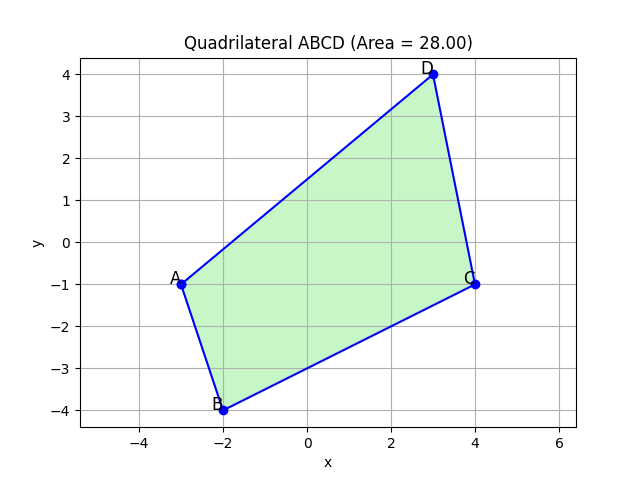
\includegraphics[height=0.5\textheight, keepaspectratio]{figs/Figure_1.png}
    \label{figure_1}
\end{figure}



\end{document}


